\documentclass{article}
\usepackage[sexy, hdr, fancy]{evan}
\usepackage{graphicx}
\usepackage{subcaption}
\usepackage{float}
\graphicspath{.}
\setlength{\droptitle}{-4em}

\DeclareMathOperator{\re}{Re}
\DeclareMathOperator{\im}{Im}

\lhead{Homework 2}
\rhead{Complex Analysis}
\lfoot{}
\cfoot{\thepage}

\begin{document}
\title{Homework 2}
\maketitle
\thispagestyle{fancy}

\section*{Section 1.6}

\begin{enumerate}[(a)]
		\ii $\abs{z-1+i}\le 3$
		\ii $\abs{\arg z} < \pi/4$
		\ii $0<\abs{z-2}<3$
		\ii $-1<\im z\le 1$
		\ii $\abs{z}\ge 2$
		\ii $(\re z)^2>1$
\end{enumerate}

\begin{itemize}
	\item[2.] Sketch each of the given sets.
		\begin{answer*}
			Plots attached on last page. All generated by me in MATLAB.
		\end{answer*}

		\begin{figure}[h]
			\begin{subfigure}{0.5\textwidth}
				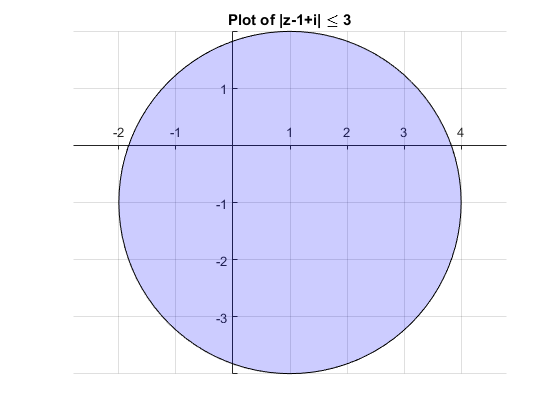
\includegraphics[width=8cm]{2a}
				\caption{Plot of $\abs{z-1+i}\le 3$}
			\end{subfigure}
			\begin{subfigure}{0.5\textwidth}
				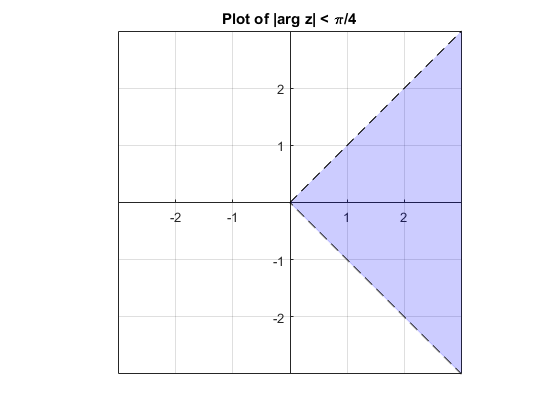
\includegraphics[width=8cm]{2b}
				\caption{Plot of $\abs{\arg z}<\pi/4$}
			\end{subfigure}
			\begin{subfigure}{0.5\textwidth}
				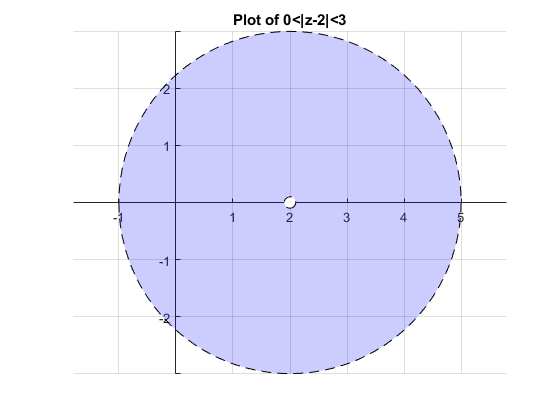
\includegraphics[width=8cm]{2c}
				\caption{Plot of $0<\abs{z-2}<3$}
			\end{subfigure}
			\begin{subfigure}{0.5\textwidth}
				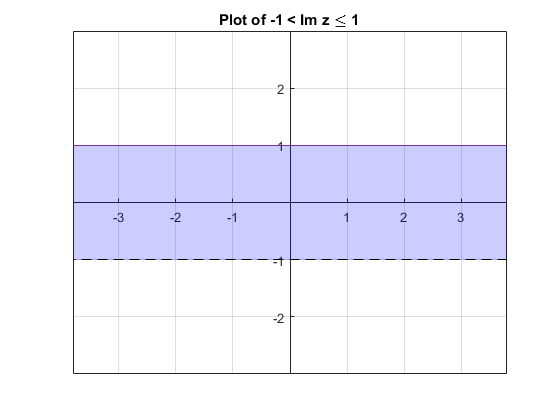
\includegraphics[width=8cm]{2d}
				\caption{Plot of $-1<\im z\le 1$}
			\end{subfigure}
			\begin{subfigure}{0.5\textwidth}
				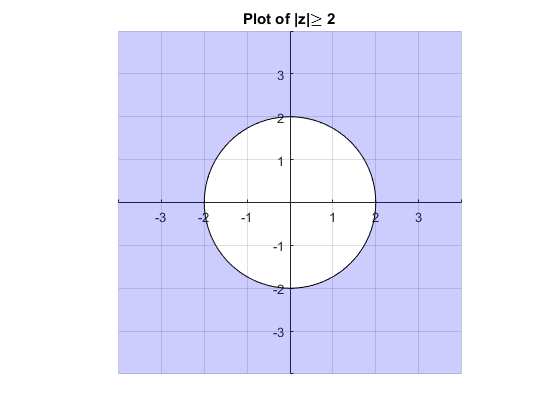
\includegraphics[width=8cm]{2e}
				\caption{Plot of $\abs{z}\ge 2$}
			\end{subfigure}
			\begin{subfigure}{0.5\textwidth}
				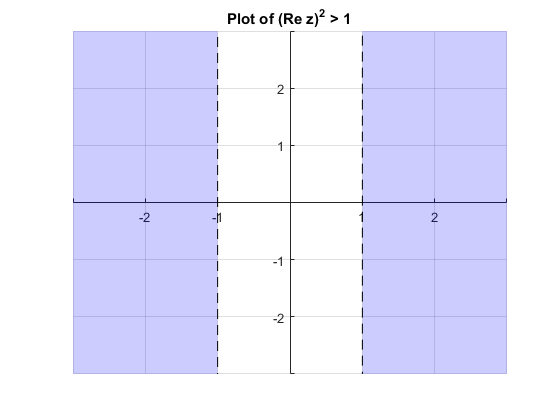
\includegraphics[width=8cm]{2f}
				\caption{Plot of $(\re z)^2>1$}
			\end{subfigure}
		\end{figure}
		
	\item[3.] Which of the given sets are open?
		\begin{answer*}
			(b), (c), (f) are open.
		\end{answer*}

	\item[4.] Which of the given sets are domains?
		\begin{answer*}
			(b), (c) are domains.
		\end{answer*}

	\item[6.] Describe the boundary of each of the given sets.
		\begin{answer*}
			(a) Solid boundary circle of radius 3 centered at $z=1-i.$

			(b) Two dotted rays from the origin, $\theta=\pi/4$ and $\theta=-\pi/4.$

			(c) Dotted boundary circle of radius 3 centered at $z=2,$ and a hole at $z=2.$
			
			(d) Solid boundary line at $\im z=1$ and dotted boundary line at $\im z=-1.$

			(e) Solid boundary circle of radius 2 centered at the origin.

			(f) Two dotted boundary lines at $\re z = 1$ and $\re z = -1.$

		\end{answer*}

	\item[extra.] Which of the sets are closed?
		\begin{answer*}
			(a), (e) are closed.
		\end{answer*}
		
\end{itemize}

\section*{Section 2.1}

\begin{itemize}
	\item[3.] Describe the range of each of the following functions.
		\begin{enumerate}[(a)]
			\item $f(z)=z+5$ for $\re z>0$
				\begin{soln}
					The range is $\left\{ z:\re z>5 \right\},$ all complex numbers with real part greater than 5.
				\end{soln}

			\item $g(z)=z^2$ for $z$ in the first quadrant, $\re z\ge 0, \im z\ge 0.$
				\begin{soln}
					Here, $z=re^{\theta i}$ with $0\le \theta\le \pi/2.$ Then $g(z)=z^2=r^2e^{2\theta i}$ where $0\le 2\theta \le \pi/2.$ Thus the range is the all of the first two quadrants.
				\end{soln}

			\item $h(z)=\frac{1}{z}$ for $0<\abs{z}\le 1$
				\begin{soln}
					The range is $\left\{ z:\abs{z}\ge 1 \right\},$ all complex numbers at least 1 away from the origin.
				\end{soln}

			\item $p(z)=-2z^3$ for $z$ in the quarter-disk $\abs{z}<1, 0<\arg z<\pi/2.$
				\begin{soln}
					Here, $z=re^{i\theta}$ with $0<\theta<\pi/2$ and $r<1.$ Then $p(z)=-2z^3=-2r^3 e^{3\theta i},$ where $0<3\theta <3\pi/2,$ and $\abs{-2r^3 e^{3\theta i}}<2.$ Thus the range is the 3/4-disk of radius 2 centered at the origin, with $0<\varphi<3\pi/2.$
				\end{soln}
				
		\end{enumerate}

	\item[5.] (e) For the complex exponential function $f(z)=e^z$ defined in Sec 1.4, describe the image of the infinite strip $0\le \im z\le \pi/4.$
		\begin{soln}
			For $z$ in this strip, we have $z=a+bi$ where $0\le b\le \pi/4.$ Then $e^z=e^{a+bi}=e^a e^{bi},$ where $e^{bi}$ lies between the rays $\theta=0$ and $\theta=\pi/4$ in the complex plane. Then $e^a$ can be any positive number, so the image is is all complex numbers with $0\le \theta\le \pi/4$ excluding 0.
		\end{soln}

	\item[6.] The Joukowski mapping is defined by
		\begin{align*}
			w=J(z) = \frac{1}{2}\left( z+\frac{1}{z} \right)
		\end{align*}
		Show that
		\begin{enumerate}[(a)]
			\item $J(z)=J(1/z)$
				\begin{proof}
					We have
					\begin{align*}
						J\left( \frac{1}{z} \right) &= \frac{1}{2} \left( \frac{1}{z} + \frac{1}{1/z} \right) = \frac{1}{2}\left( \frac{1}{z} + z \right) = J(z)
					\end{align*}
				\end{proof}

			\item $J$ maps the unit circle $\abs{z}=1$ onto the real interval $[-1, 1].$
				\begin{proof}
					We have
					\begin{align*}
						J(z) &= \frac{1}{2}\left( z+\frac{1}{z} \right) = \frac{1}{2} \left( z+\frac{\overline z}{\abs{z}^2} \right) = \frac{1}{2}\left( z+\overline z \right) = \re z
					\end{align*}
					for $z$ on the unit circle, which is the range $[-1, 1].$
				\end{proof}

			\item $J$ maps the circle $\abs{z}=r\quad (r>0, r\neq 1)$ onto the ellipse
				\begin{align*}
					\frac{u^2}{\left[ \frac{1}{2}\left( r+\frac{1}{r} \right) \right]^2} + \frac{v^2}{\left[ \frac{1}{2}\left( r-\frac{1}{r} \right) \right]^2} = 1
				\end{align*}
				which has foci at $\pm 1.$
				\begin{proof}
					Let $z=r(\cos \theta + i\sin \theta).$ Then
					\begin{align*}
						J(z) &= \frac{1}{2} \left[ r(\cos \theta + i\sin \theta) + \frac{1}{r(\cos \theta + i\sin \theta)} \right] \\
						&= \frac{1}{2}\left[ r(\cos \theta + i\sin \theta) + \frac{1}{r} (\cos \theta - i\sin \theta) \right] \\
						&= \frac{1}{2}\left( r+\frac{1}{r} \right)\cos \theta + i\cdot\frac{1}{2}\left( r-\frac{1}{r} \right)\sin \theta
					\end{align*}
					If we treat this as a parametric equation in $\RR^2$ where $u=\frac{1}{2}\left( r+\frac{1}{r} \right)\cos \theta$ and $v = \frac{1}{2}\left( r-\frac{1}{r} \right)\sin \theta,$ this traces out the ellipse
					\begin{align*}
						1 &= \cos^2\theta+\sin^2\theta = \left( \frac{u}{\frac{1}{2}\left( r+\frac{1}{r} \right)} \right)^2 + \left( \frac{v}{\frac{1}{2}\left( r-\frac{1}{r} \right)} \right)^2
					\end{align*}
					as desired. The foci $c$ satisfy
					\begin{align*}
						c^2 &= \left[ \frac{1}{2}\left( r+\frac{1}{r} \right) \right]^2 - \left[ \frac{1}{2}\left( r-\frac{1}{r} \right) \right]^2 = \frac{1}{4}\left[ \left(r^2+\frac{1}{r^2} + 2\right) - \left( r^2+\frac{1}{r^2} - 2 \right)  \right] = 1 \\
						\implies c &= \pm 1
					\end{align*}
				\end{proof}

		\end{enumerate}
		
\end{itemize}

\section*{Section 2.2}

\begin{itemize}
	\item[2.] Sketch the first five terms of the sequence $(2i)^n, n=1, 2, 3, \cdots$ and then describe the divergence of this sequence.
		\begin{soln}
			This graph was generated in MATLAB. The divergence goes to infinity.
			\begin{figure}[H]
				\centering
				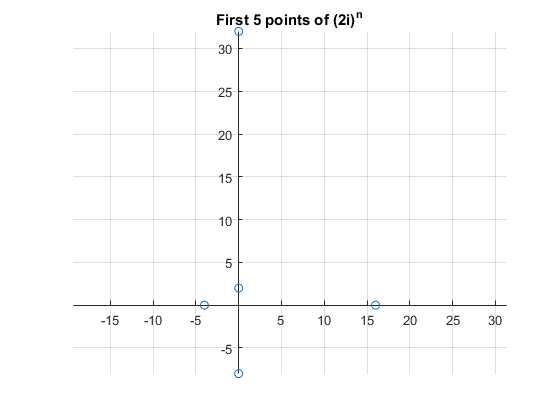
\includegraphics[width=10cm]{seq}
				\caption{First 5 points of $(2i)^n$}
			\end{figure}
			
		\end{soln}

	\item[7.] Decide whether each of the following sequences converges, and if so, find its limit.
		\begin{enumerate}[(a)]
			\item $z_n=\frac{i}{n}$
				\begin{soln}
					This sequence converges to 0.
				\end{soln}

			\item $z_n=i(-1)^n$
				\begin{soln}
					This sequence does not converge because it oscillates between $i$ and $-i.$
				\end{soln}

			\item $z_n=\arg\left( -1+\frac{i}{n} \right)$
				\begin{soln}
					We have 
					\begin{align*}
						z_n &= \arg\left( -1+\frac{i}{n} \right) = \tan\inv\left( \frac{1}{n} \right) \to 0
					\end{align*}
					Since the complex number is in the second quadrant, $z_n\to \pi.$
				\end{soln}

			\item $z_n=\frac{n(2+i)}{n+i}$
				\begin{soln}
					We have
					\begin{align*}
						z_n &= \frac{n(2+i)}{n+i} = \frac{(2n+ni)(n-i)}{n^2+1} = \frac{(2n^2+n) + (n^2-2n)i}{n^2+1} \\
						&= \frac{2n^2+n}{n^2+1} + \frac{n^2-2n}{n^2+1}i \to 2 + i
					\end{align*}
					so the sequence converges to $2+i.$
				\end{soln}

			\item $z_n=\left( \frac{1-i}{4} \right)^n$
				\begin{soln}
					We have
					\begin{align*}
						z_n &= \left( \frac{1}{4} \right)^n (1-i)^n = \left( \frac{\sqrt{2}}{4} \right)^n \left( \frac{1}{\sqrt{2}} - \frac{1}{\sqrt{2}}i \right)^n \\
						&= \left( \frac{\sqrt{2}}{4} \right)^n e^{-n\pi i/4} \to 0
					\end{align*}
					so this sequence converges to 0.
				\end{soln}
				
			\item $z_n=\exp\left( \frac{2n\pi i}{5} \right)$
				\begin{soln}
					This sequence does not converge because it oscillates between 10 distinct values.
				\end{soln}
				
		\end{enumerate}

	\item[21.] (d) Find the limit
		\begin{align*}
			\lim_{z\to-\pi i} \exp\left( \frac{z^2+\pi^2}{z+\pi i} \right)
		\end{align*}
		\begin{soln}
			We have
			\begin{align*}
				\lim_{z\to-\pi i} \exp\left( \frac{z^2+\pi^2}{z+\pi i} \right) &= \lim_{z\to-\pi i} \exp\left( \frac{(z+\pi i)(z-\pi i)}{z + \pi i} \right) \\
				&= \lim_{z\to-\pi i} e^{z-\pi i} = e^{-2\pi i} = 1
			\end{align*}
		\end{soln}
		
\end{itemize}

\end{document}
